% LambdaCube-CL.tex
\begin{hcarentry}[updated]{LambdaCube}
\report{Csaba Hruska}%05/12
\status{experimental, active development}
\makeheader

LambdaCube 3D is a domain specific language and library that makes it
possible to program GPUs in a purely functional style.

Programming with LambdaCube constitutes of composing a pure data-flow
description, which is compiled into an executable module and accessed
through a high-level API.  The language provides a uniform way to
define shaders and compositor chains by treating both streams and
framebuffers as first-class values.

In its current state, LambdaCube is already functional, but still in
its infancy.  The current API is a rudimentary EDSL that is not
intended for direct use in the long run.  It is essentially the
internal phase of a compiler backend exposed for testing purposes.  To
exercise the library, we have created two small proof of concept
examples: a port of the old LambdaCube Stunts example, and a Quake III
level viewer.

Over the last few months, we extended the implementation with some
essential major features:

\begin{itemize}
\item texture support
\item multi-pass rendering
\item sharing detection and CSE in the shaders (through hash-consing)
\end{itemize}

We also improved the existing examples and created new ones: a
showcase for variance shadow mapping and another for integration with
the Bullet physics engine.

Last but not least, we finally started a new blog dedicated to
LambdaCube.  The blog is intended to be the primary source of
information and updates on the project from now on.

Everyone is invited to contribute! You can help the project by playing
around with the code, thinking about API design, finding bugs (well,
there are a lot of them anyway), creating more content to display, and
generally stress testing the library as much as possible by using it
in your own projects.

%**<img width=500 src="./lc-q3.png">
%*ignore
\begin{center}
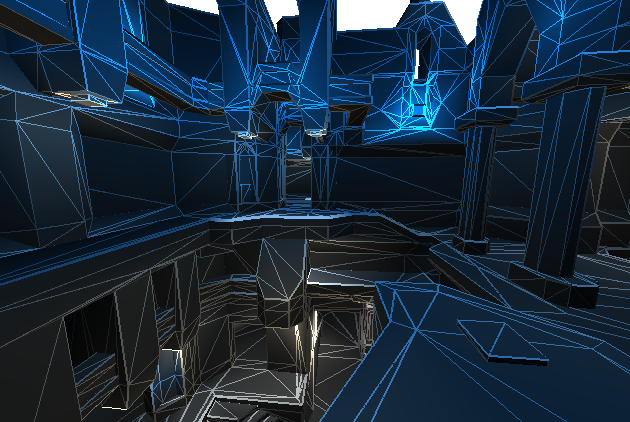
\includegraphics[width=0.47\textwidth]{html/lc-q3.png}
\end{center}
%*endignore

\FurtherReading
\begin{compactitem}
\item \url{https://lambdacube3d.wordpress.com/}
\item \url{https://github.com/csabahruska/lc-dsl}
\item \url{http://www.haskell.org/haskellwiki/LambdaCubeEngine}
\item \url{http://www.youtube.com/watch?v=kDu5aCGc8l4}
\end{compactitem}
\end{hcarentry}
